\section{Fissione e Fusione Nucleare}

\subsection{Fissione Nucleare}
\paragraph{Fissione spontanea}
Perché tutti gli elementi con numero di massa elevato non decadono spontaneamente in $^{56}Fe$?

Quando si è parlato della formula semiempirica di massa, si è visto che una delle logiche di funzionamento della natura è che la somma dei protoni e neutroni legati è minore della somma dei pesi degli elementi slegati. 
La differenza di massa è l'energia di legame
\[
\Delta mc^2=BE.
\]
Essendo che il ferro come abbiamo visto è l'elemento con l'energia di legame maggiore, è lecito chiedersi cosa blocchi un eventuale decadimento dei nuclei più pesanti nel ferro in quanto energeticamente favorevole (massimizzando l'energia di legame minimizzo l'energia di massa).
\[
A\to A/2?
\]
Per passare da uno stato $A$ legato a due nuclei $A/2$ bisogna necessariamente per uno stato intermedio di un nucleo deformato dove sono presenti due nuclei legati tra loro ma identificati.
Studiamo quindi questo stato intermedio 
\begin{equation}
BE= a_v A-a_s A^{2/3}-a_c \frac{Z(Z-1)}{A^{1/3}}-a_{sym}\frac{(N-Z)^2}{A}+\delta_p
\end{equation}
In questo caso ignoriamo quello che è il termine di accoppiamento $\delta_p$ considerando il caso di due nuclei \emph{even-even}.
Vogliamo confrontare l'energia di legame del nucleo unico (1) al caso del nucleo quasi separato (2).

Il termine di volume sarà:
\begin{enumerate}
\item $a_v A$
\item $2a_v \frac{A}{2}$
\end{enumerate}
Questi due termini sono uguali, il che non è sorprendente perché il modello a goccia mantiene costante il volume.

Prendiamo ora il termine di simmetria:
\begin{enumerate}
\item $a_{sym}\frac{(N-Z)^2}{A}$
\item $a_{sym} 2\biggl[\frac{(N/2 -Z/2)^2}{A/2}=a_{sym}\frac{(N-Z)^2}{A}$
\end{enumerate}
Nemmeno questo termine varia.

Consideriamo il termine di superficie:
\begin{equation}
V_1=V_2\to \frac{4}{3}\pi R^3=2\frac{4}{3}\pi r^3
\end{equation}
\begin{equation}
R^3=2r^3\to R=1,26 r
\end{equation}
\begin{enumerate}
\item $S_1=4\pi R^2=4\pi(1,26)^2r^2=6\pi r^2$
\item $S^2=2\cdot 4\pi r^2=8\pi r^2$
\end{enumerate}
Se deformiamo un nucleo la superficie aumenta, il che comporta un aumento del termine di superficie e quindi una diminuzione dell'energia di legame.

Vediamo dunque come si comporta il termine coulombiano:
\begin{enumerate}
\item $V_1=\frac{a_c Z(Z-1)}{A^{1/3}}$
\item $V_2= \frac{2(a_c Z/2 (Z/2-1))}{(a/2)^{1/3}}=\frac{1,26\cdot2}{4}\frac{a_c Z(Z-2)}{a^{1/3}}$
\end{enumerate}
Da un confronto con nuclei ad alto Z, la differenza tra $Z-1$ e $Z-2$ è trascurabile
\begin{equation}
V_2\sim \frac{2}{3} v_1
\end{equation}
In questo caso si ha che il termine coulombiano diminuisce con la formazione dello stato intermedio, il che comporta un aumento dell'energia di legame.

Qual è quindi il termine dominante in questa fase intermedia?

Posso prendere come riferimento i valori che erano stati trovati dei termini
\[
a_c=0,7MeV \hspace{0.2cm}a_s=18MeV
\]
Il termine dominante è quindi il termine di superficie, si ha quindi che nella fase intermedia l'energia di legame diminuirà, portando ad un'energia di massa maggiore, creando così una barriera di potenziale.
Per questo è impossibile una fissione spontanea dei nuclei più pesanti del Ferro.
La $\Delta E\approx 6MeV$ tra il nucleo legato e lo stato intermedio è chiamata \emph{energia di attivazione}.
I nuclei che fanno fissione spontanea sono i nuclei che hanno 
\begin{equation}
\frac{Z^2}{A}>51
\end{equation}

\paragraph{Fissione Indotta}
La differenza energetica evidenziata nel primo paragrafo corrisponde più esattamente a 
\begin{equation}
\Delta E=6,2MeV
\end{equation}
Il processo sfruttato è quello di inviare neutroni su nuclei di Uranio, il primo a effettuare questo processo fu Fermi che però non riconobbe il fenomeno.
\begin{equation}
n+^{235}U\longrightarrow X+Y+Nn+Q
\end{equation}
Il pensiero più logico è quello che in questo processo per superare l'energia di attivazione si debba prendere un neutrone abbastanza energetico che trasferisca l'energia di attivazione necessaria a far cominciare il processo.
\begin{figure}[h]
\centering
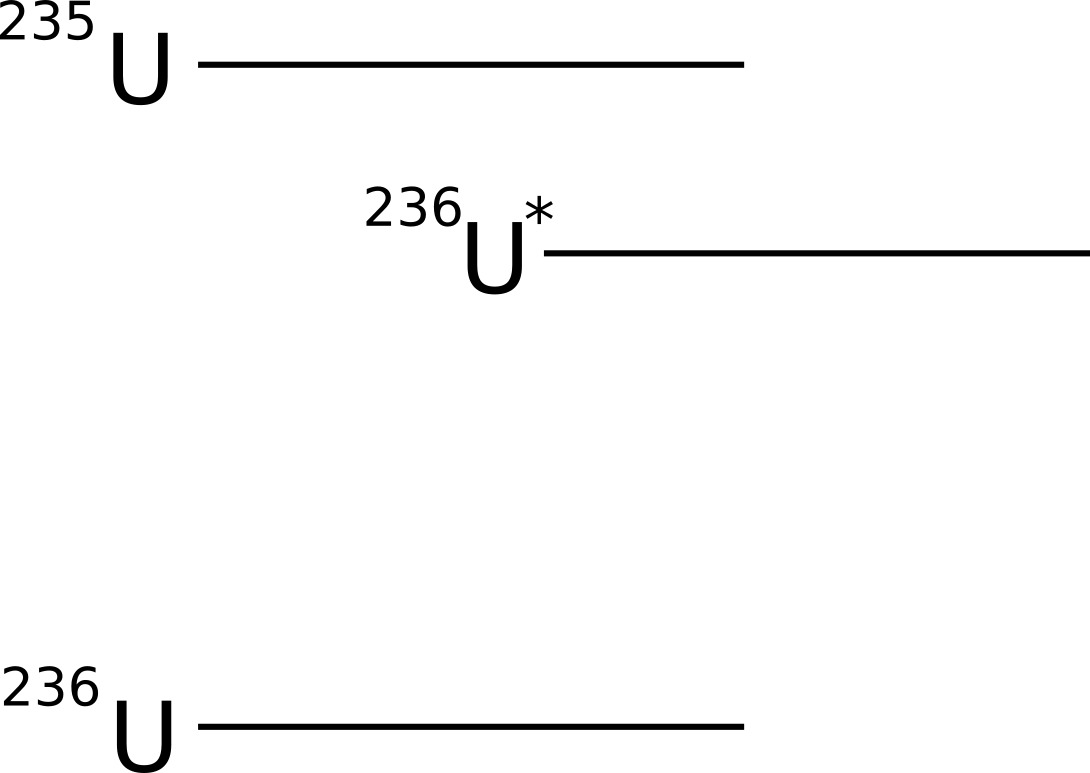
\includegraphics[width=120pt]{fig6_01}
\caption{Livelli che interessano la fissione indotta dell'uranio 235.}
\end{figure}

In realtà si è visto che questo tipo di fenomeno si verifica con neutroni termici (ovvero neutroni a temperatura ambiente) che possiedono quindi energia pari a 
\begin{equation}
E=KT=\SI{9e-5}{\frac{eV}{K}}\times 300K=\SI{27e-3}{eV}
\end{equation}
Un'energia molto minore all'energia di attivazione!

Quello che si verifica è che un neutrone termico assorbito dall'Uranio da origine ad un atomo di Uranio 236 in uno stato eccitato con energia maggiore dell'energia di attivazione.
\begin{equation}
n+^{235}U\to ^{236}_{92}U*
\end{equation}

Da notare che in natura la composizione dell'uranio è
\[
^{238}U\hspace{0.1cm} al\hspace{0.1cm} 99,28\%\hspace{0.5cm}^{235}U\hspace{0.1cm} al\hspace{0.1cm} 0,72\%
\]
E nel caso dell'uranio 238 lo stato che si viene a formare dopo l'assorbimento di un neutrone ha energia pari a $4,8MeV$ che non basta per innescare il decadimento, per processi di fissione nucleare viene quindi sfruttato solamente $^{235}U$.
Dal punto di vista fisico questo si rappresenta tramite la sezione d'urto.

Facendo un grafico della sezione d'urto si ha che questa, partendo da un valore iniziale di $500b$, diminuisce aumentando l'energia.
Questo effetto è dovuto al fatto che aumentando l'energia è vero che si supera più facilmente la barriera di potenziale ma sarà anche più difficile mantenere nel nucleo il neutrone che tenderà invece a fuggire.
\'E quindi conveniente usare i neutroni a più bassa energia disponibili alla fissione.
Il bilancio energetico per cattura neutronica da $^{235}U$ e $^{238}U$ è dovuto al termine di accoppiamento $\delta _q$ nella formula semiempirica di massa, infatti, mentre l'uranio 235 ha un numero dispari di neutroni che comporta una tendenza ad assorbire un neutrone per pareggiare il livello energetico, l'uranio 238 ha un numero pari di entrambi gli elementi che porta ad una stabilità che evita l'assorbimento neutronico spontaneo (non c'è quindi l'energia addizionale di accoppiamento).

Qual è la distribuzione di massa dei prodotti di reazione?
La previsione fatta era che i nuclei si dividessero come:
\[
A\longrightarrow 2A/2
\]
In questo caso la formula semiempirica di massa fa una predizione sbagliata infatti è stato verificato sperimentalmente che per esempio i nuclei di uranio hanno la tendenza a produrre con maggior frequenza nuclei con numeri di massa in distribuzione gaussiana attorno a $A=95,140$ con un minimo centrale tra i due picchi a $A=118$.

In questo caso ciò che subentra è il modello a shell, i nuclei generati tenderanno ad addensarsi attorno ai nuclei che abbiamo visto essere più stabili nel modello a shell nucleonico.
I nuclei figli che si trovano ad avere più neutroni rispetto alle valli di stabilità tenderanno a decadere $\beta^-$ per tornare in uno stato stabile.

Restando in questo argomento dei prodotti di fissione prendiamo un caso particolare:
\begin{equation}
n+^{235}U \longrightarrow ^{236}U*\longrightarrow^{140}_{54}Xe+^{94}_{38}Sr+2n
\end{equation}
I modi di fissione dell'uranio sono vari e un ingegnere di una centrale nucleare deve conoscerli tutti. In questo caso il processo non si ferma lì ma decadono pure i nuclei figli con un processo di decadimento $\beta^-$:
\begin{equation}
\begin{split}
^{140}_{54}Xe &\longrightarrow ^{140}_{55}Cs \longrightarrow ^{140}_{56}Ba \longrightarrow ^{140}_{57}La \longrightarrow ^{140}_{58}Ce\\
^{94}_{38}Sr&\longrightarrow^{94}_{39}Y \longrightarrow^{94}_{40}Zr
\end{split}
\end{equation}
Un altro modo di decadimento è:
\begin{equation}
^{236}U\longrightarrow^{137}_{53}I+^{97}Y+2n+Q
\end{equation}
In questo caso lo Xeon decade come:
\begin{equation}
^{137}_{53}I \longrightarrow^{137}_{54}Xe\longrightarrow^{136}_{54}Xe+n
\end{equation}
Lo Xeon è essenziale per il funzionamento delle centrali nucleari e in particolare quest'ultimo processo che porta all'emissione di neutroni è fondamentale nel controllo del reattore.

Il processo di fissione avviene con un tempo caratteristico di $t=10^{-12}s$.
I neutroni emessi nel processo principale vengono chiamati \emph{neutroni prompt}, quelli che invece vengono generati nei processi di decadimento sono chiamati \emph{neutroni ritardati}.
Quest'ultimi sono ciò che tiene sotto controllo il reattore nucleare e se non ci fossero non saremmo in grado di far funzionare i reattori.
I neutroni prompt sono invece quelli fondamentali alla produzione di energia.

\paragraph{Principi di funzionamento di un reattore nucleare a fissione}
Abbiamo visto che la fissione dell'$^{235}U$ avviene con un processo del tipo
\begin{equation}
n+^{235}U\longrightarrow^{236}U*\longrightarrow X+Y+2n+Q
\end{equation}

Un reattore nucleare è formato da un contenitore che scherma dalle radiazioni emesse dai prodotti di reazione.
All'interno sono poste le barre di combustibile ovvero di materiale reagente.
Per raccogliere il calore il contenitore è pieno di liquido refrigerante, normalmente di acqua, che attraverso delle condutture viene raccolta e convogliata attraverso uno scambiatore di calore che invia poi l'acqua all'interno del reattore.
Il meccanismo di raffreddamento dell'acqua e quindi di produzione energetica è uguale a quello di qualsiasi altra centrale elettrica, ciò che cambia è solamente il metodo di riscaldamento.
 
 Ci sono due tipi di problemi che si presentano all'interno di un reattore:
\begin{enumerate}
\item \textbf{Dobbiamo rallentare i neutroni.} 
I neutroni prodotti nella reazione non sono a energia termica e abbiamo visto che se vogliamo massimizzare la sezione d'urto di cattura dobbiamo diminuire la velocità e portare i neutroni all'energia adeguata.
\item \textbf{Dobbiamo ridurre n a 1.} 
Mediamente il numero di neutroni per fissione è di 2,5 e quindi se non c'è controllo di reazione si ha che ogni 2 reazioni generano in media 5 reazioni. 
Questo non va bene perché porta fuori controllo il reattore che diventa una bomba.
Cerchiamo di avere un rapporto di 1 a 1 tra le reazioni.
\end{enumerate}

Le soluzioni che permettono quindi il corretto funzionamento del reattore sono:
\begin{enumerate}
\item \textbf{Determinazione del moderatore.}
\begin{figure}[h]
\centering
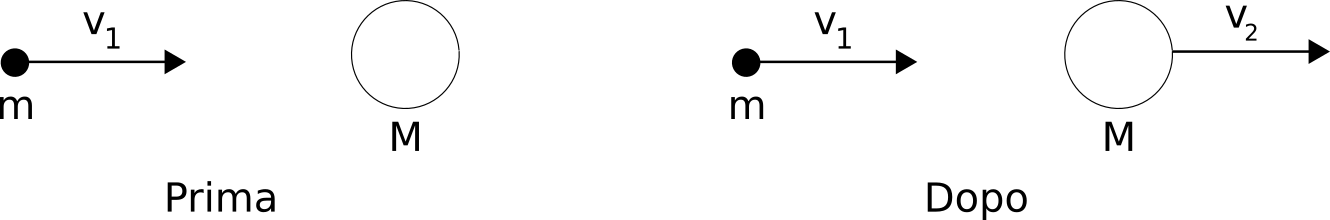
\includegraphics[width=220pt]{fig6_02}
\caption{Interazione di un nucleo con un neutrone}
\end{figure}

Per la conservazione della quantità di moto si ha 
\begin{equation}
\begin{split}
p=cost\hspace{1cm}&mv=mv_1+Mv_2\\
K=cost\hspace{1cm}&\frac{1}{2}mv^2=\frac{1}{2}mv_1^2+\frac{1}{2}Mv_2^2\\
&v_2=\frac{m}{M}(v-v_1)\\
&v_2^2=\frac{m}{M}(v^2-v_1^2)
\end{split}
\end{equation}
Le due formule ottenute sopra possono essere combinate per ottenere 
\begin{equation}
\begin{split}
\frac{m}{M}(v^2-v_2^2)&=\frac{m}{M}(v-v_1)^2\\
Mv^2-Mv_1^2&=m(v-v_1)^2\\
M(v-v_1)(v+v_1)&=m(v-v_1)^2\\
Mv+Mv_1&=mv-mv_1
\end{split}
\end{equation}
Si può quindi ricavare $v_1$ da questa formula ottenendo
\begin{equation}
v_1=v\frac{m-M}{m+M}
\end{equation}
Si può cercare di minimizzare questa velocità per trovare con che materiale si possa termalizzare i neutroni.
La condizione è semplice da vedere:
\[
m\sim M
\]
Il miglior materiale che utilizza il minor numero di urti per rallentare il neutrone è quindi quello che ha massa uguale a quella del neutrone.
Il materiale più utilizzato è l'acqua che presenta caratteristiche termiche ideali, ma soprattutto presenta le caratteristiche ideali per il rallentamento dei neutroni.
L'acqua non è quindi solamente un refrigerante ma anche un moderatore.

\item \textbf{Riduzione dei neutroni prodotti da $N=2,5\to 1$.}

In questo caso possono esserci più modi e in alcuni casi la natura ci viene in contro.
\begin{itemize}
\item Alcuni neutroni vengono assorbiti senza produrre fissione, può accadere infatti che l'Uranio 236 si disecciti tramite emissione $\gamma$.

In questo caso il parametro che ci è utile è $\eta$ che corrisponde alla frazione di neutroni che sopravvive all'assorbimento ($\eta<1$).

\item Il secondo effetto è che alcuni neutroni veloci possono produrre fissione nel Uranio 238 $^{238}U$, infatti anche se nelle centrali viene usato dell'uranio arricchito la percentuale più alta ($97\%$)è di uranio 238.

Per questo effetto teniamo conto di un fattore $\varepsilon$ che corrisponde alla frazione di neutroni prodotti da fissione in $^{238}U$ ($\varepsilon>1$ quindi questi neutroni ne producono comunque altri).

\item Nel grafico della sezione d'urto in funzione dell'energia esiste una regione tra $1\to 100eV$ chiamata \emph{regione delle risonanze}, in cui vengono assorbiti neutroni che vengono eliminati dal ciclo (senza riuscire a termalizzare).

Questo effetto è regolato da $p$ che corrisponde alla frazione di neutroni che sopravvive alle risonanze($p<1$).

\item I neutroni possono essere assorbiti dal moderatore.

Questo viene chiamato fattore $f<1$, in particolare un neutrone può essere assorbito da un protone dell'acqua dando luogo ad un deutone, trasformando quindi l'acqua in quella che viene chiamata acqua pesante.
\[
H_2O\to D_2O
\]
Tra l'altro l'utilizzo dell'acqua pesante come moderatore non ne varia l'efficacia, si abbassa anzi la probabilità che vengano assorbiti neutroni.
Esistono quindi delle centrali che vengono raffreddate e moderate con acqua pesante.
\end{itemize}
Si ha quindi che la frazione di neutroni che sopravvive a questi effetti è dato dalla \emph{formula dei quattro fattori}
\begin{equation}
N=N\eta\varepsilon p f=KN
\end{equation}
introdotta da Fermi.
Per il corretto funzionamento del reattore devo mantenere $K=1$.
\end{enumerate}

\paragraph{Controllo del reattore}

\textbf{Esempio}\\
Si abbia
\[
K=1+\delta\hspace{0.5cm}\delta=0,01
\]
I tempi caratteristici della fissione sono $t=10^{-12s}$ che corrisponde al tempo di fissione, seguito poi dal tempo di rallentamento dei neutroni per la generazione di una seconda fissione $t=10^{-3}s=\tau$.

Supponendo che il processo vada avanti per $t$ secondi, il numero di cicli sarà dato da 
\begin{equation}
n=\frac{t}{\tau}
\end{equation}
Dobbiamo considerare che per ogni interazione il numero di neutroni cresce di $1+\delta$.
L'evoluzione dei neutroni è descritta come
\begin{equation}
N(t)=N(0)(1+\delta)^{t/\tau}
\end{equation}
dove $N(x)$ è il numero di neutroni dopo il tempo x, $K=1+\delta$ è il numero di neutroni che si producono ad ogni interazione.
Facendone il logaritmo sin ottiene
\begin{equation}
\ln N(t)=\ln N(0)+\ln(1+\delta)+\frac{t}{\tau}
\end{equation}
Se $\delta$ è piccolo si ha
\begin{equation}
\ln N(t)=\ln N(0)+\frac{t}{\tau}\delta
\end{equation}
Facendo l'esponenziale si trova
\begin{equation}
N(t)=N(0)e^{\frac{t\delta}{\tau}}
\end{equation}
Dopo un tempo $t=1s$ ottengo 
\begin{equation}
N(1)=N(0)e^10
\end{equation}
Si ha quindi un fattore moltiplicativo di $\sim 22026$. E questo descrive un processo controllato il che ci fa comprendere come sia essenziale un controllo efficace di $K$.

Per il controllo  di un reattore oltre al combustibile e al liquido refrigerante bisogna inserire anche delle barre di controllo che assorbono neutroni (per esempio un ottimo materiale di controllo è il cadmio $Cd$).

Un reattore può essere:
\begin{equation}
\begin{split}
&K=1\hspace{1cm}critico\\
&K<1\hspace{1cm}sottocritico\\
&K>1\hspace{1cm}supercritico
\end{split}
\end{equation}
Essendo il tempo di rallentamento dell'ordine del millisecondo, questo non è compatibile con il tempo meccanico di inserimento di queste barre, ma come abbiamo visto il fattore $k$ richiede una precisione estrema perché anche delle piccole variazioni del sistema potrebbero portare ad un collasso rapido.

Per questo vengono in aiuto i \emph{neutroni ritardati}, che vengono sfruttati per portare il reattore a $K=1$ (situazione di criticità).
La reazione che produce i neutroni ritardati come abbiamo visto avviene in un tempo di qualche secondo, questo permette l'inserimento delle barre in un tempo adatto al controllo.

\paragraph{Tipi di Reattori}
\begin{enumerate}
\item \emph{Reattore ad acqua in pressione (PWR).} 
Questo vuol dire che l'acqua all'interno del reattore è sempre nello stato liquido. 
Se infatti portiamo la pressione ad un valore di $100 atm$ allora la temperatura di ebollizione sarà di $300^oC$.
L'acqua viene fatta uscire dal reattore ad una temperatura di $250^oC$ e immessa nello scambiatore dove vaporizza acqua che andrà in forma di vapore ad azionare le turbine come in una qualsiasi altra centrale.
In questo tipo di reattore c'è la necessità di uranio arricchito.

\item \emph{Reattore ad acqua pesante(PHWR).}
In questo caso si usa al posto dell'acqua normale acqua formata con deuterio invece che idrogeno.
Il vantaggio sta nel fatto che per la proprietà di basso assorbimento di neutroni dell'acqua pesante è possibile usare Uranio naturale senza quindi il processo di arricchimento.

\item \emph{Reattore ad acqua bollente(BWR).}
In questo caso l'acqua nel circuito di scambio viene portata ad ebollizione. Si ha che quindi l'acqua del reattore viene portata ad ebollizione.

\item \emph{Reattore con moderatore a grafite.}
In questi reattori viene usata la grafite come moderatore e l'anidride carbonica come refrigerante.
\end{enumerate}

Esistono inoltre altri materiali fissili, infatti tutti i nuclidi della stessa zona dell'uranio con neutroni dispari può innescare una reazione di fissione (per esempio il plutonio 239 $^{239}Pu$ o l'uranio 233 $^{233}U$).
La peculiarità di questo è che l'uranio 238, quando cattura un neutrone, da luogo ad uno stato eccitato dell'uranio 239 che decade in Nettunio 239, che a sua volta decade il plutonio 239.
\begin{equation}
n+ ^{238}U\to ^{239}U*\to ^{239}Np\to ^{239}Pu
\end{equation}
Si ha quindi che alcune catene di reazioni portano da un combustibile ad un altro combustibile.
Un'altra catena possibile è 
\begin{equation}
n+^{232}Th\to ^{233}Th*\to ^{233}Pu\to ^{233}U
\end{equation}





